\documentclass{article}
\usepackage[T1]{fontenc}
\usepackage{lmodern}
\usepackage{graphicx}
\usepackage{amsmath,amssymb}
\usepackage[a4paper,margin=2cm]{geometry}
\usepackage[absolute,overlay]{textpos}
\setlength{\TPHorizModule}{1mm}
\setlength{\TPVertModule}{1mm}
\usepackage[indonesian]{babel}
\usepackage{hyperref}
\setlength{\emergencystretch}{2em}
% unit: Halaman 83

\begin{document}

% === Halaman 83 (llm) ===

% (tidak ada teks dari model)

% deskripsi: Grafik batang yang menunjukkan nilai numerik untuk berbagai kategori yang diberi label dua huruf (AN, AT, ED, EN, ER, ES, HE, IN, ON, OR, RE, ST, TE, TH, TI). Nilai tertinggi adalah TH dengan 3.21 dan terendah adalah ST dengan 1.22.
% bbox normalisasi: [0.1050, 0.1560, 0.9500, 0.7500]
\begin{textblock*}{177.45mm}(22.05mm,46.33mm)
\noindent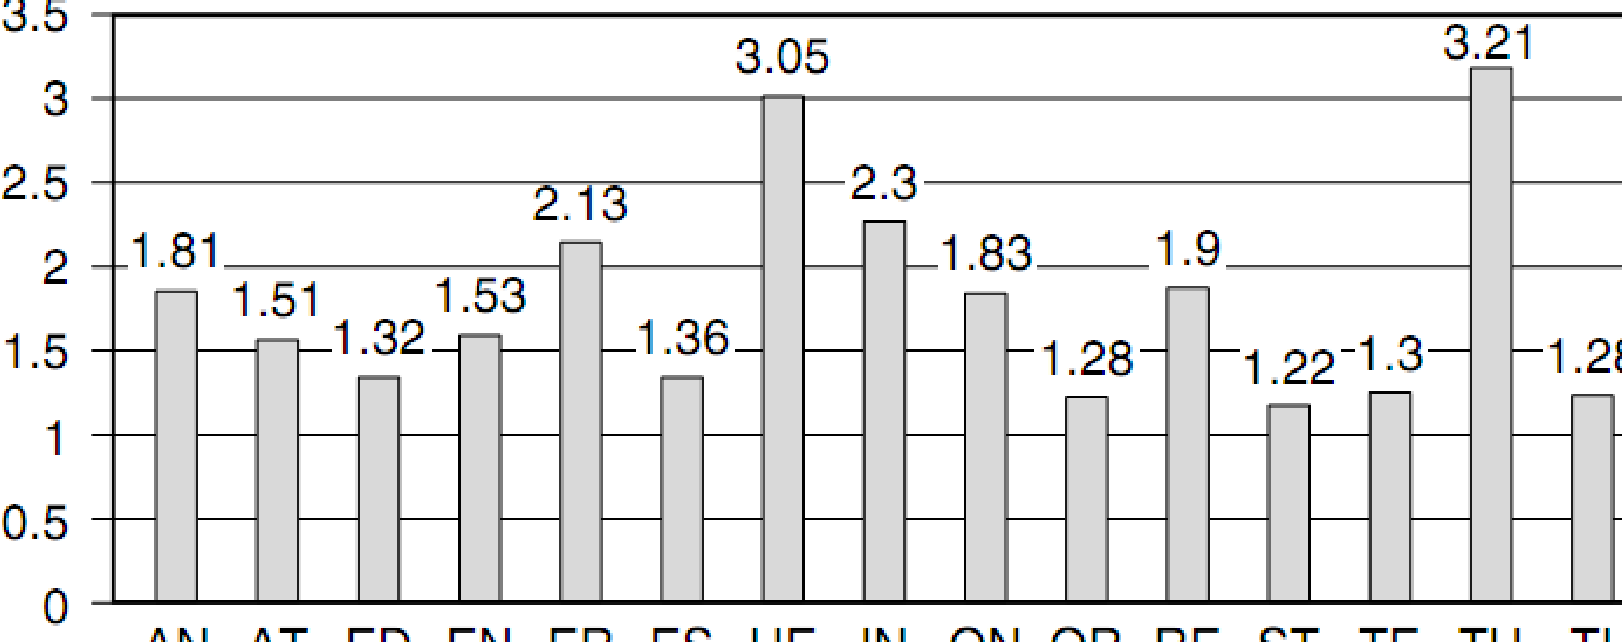
\includegraphics[width=177.45mm,height=176.42mm]{../../images/llm/page_083_img_01.png}%
\end{textblock*}

\end{document}
